\procTitle{Гранаты в породах Велиткенайского гранит-мигматитового массива (арктическая Чукотка)}
\procAuthor{Ползуненков~Г.\,О.}
\procEmail{gennadiy\_mag@mail.ru}
\procOrganization{СВКНИИ ДВО РАН} \procCity{Магадан}

\makeProcTitle
\index{p@Ползуненков~Г.\,О.}

Исследован состав гранатов в меловых породах гранит-мигматитового Велиткенайского массива (35A~--- диатектит, 41C~--- деформированный биотитовый гранит, 3300~--- гранат-мусковитовых аплит, Vel-1~--- деформированный биотитовый гранит) и вмещающих его неопротерозойских породах (12~--- метапелит, 5301A~--- гранатовое габбро).  Формирование гранатов может отражать три различных процесса эволюции пород: 1) региональный метаморфизм эпидот-амфиболитовой фации, проявленный во вмещающих неопротерозойских породах и диатектитах; 2) глубинную антекристовую магматическую кристаллизацию гранит-монцонитого расплава; 3) метаморфизм эпидот-зеленосланцевой фации в мегаксенолитах глубинных офиолитовых комплексов при их выведении на поверхность.

Традиционно принимается, что преобладание той или иной доли миналов в гранатах отражает в какой-то степени  условия его образования.  Так, в составе метаморфических гранатов  (средние до высоких фаций метаморфизма) преобладает альмандиновый компонент. Связанные с процессами метаморфизма карбонатные породы и метасоматические образования характеризуются гроссуляром. Вариации температур и давлений при метаморфизме отражаются  в содержании пиропового минала в гранатах, увеличение которого приводит к повышению температур и (или) давлений. Низкотемпературные фации метаморфизма характеризуются гранатами спессартитового состава.

Химический состав изученных гранатов определялся автором на микрозонде Camebax в СВКНИИ ДВО РАН.

Пересчёт составов на кристаллохимические формулы выполнен катионным методом. Минальный состав гранатов получен путём расчёта из формульных коэффициентов. По~химическому составу исследованные гранаты представлены группами Mg-Fe и Ca гранатов. Группа Mg-Fe гранатов в образцах представлена  скелетными порфиробластами с многочисленными включениями других минералов, не  зональными~--- от ядер к краям не происходит значимых изменений Mg, Fe, Сa, Mn (рис.1,А). Ca гранаты в гранатовом габбро 5301-A представлены симплектитами с плагиоклазом (рис. 1,Б).  В таких случаях, из-за отсутствия четких  краевых и  центральных частей у зёрен граната, анализ зональности малоэффективен и нами не проводился.

\begin{figure}[H]
  \begin{center}
    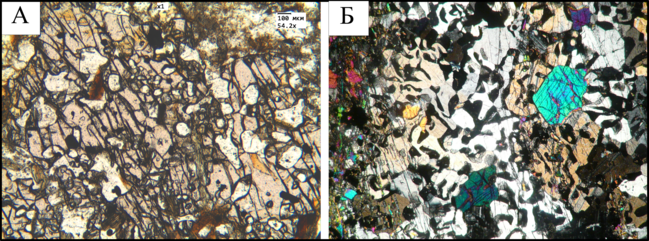
\includegraphics[width=0.6\textwidth]{authors/polzunenkov-fig1.png}
  \end{center}
  \caption {Микрофотографии выделений гранатов в шлифах: A~--- порфилобласт из обр. 12; \\Б~--- симплектитовые выделения в обр. 5301-A
}

\end{figure}


По соотношению рассчитанных миналов (рис. 2) Mg-Fe гранаты представлены альмандинами, подразделяющимися по содержанию пиропового минала на высокопиропистые (обр. 12, 35A~--- Prp $\sim$18\,\%  ) и низкопиропистые (обр. 3300, 41C, Vel-1~--- Prp\,<\,7\,\% ), а Ca гранаты представлены гросcуляром с повышенным содержанием андрадитового минала (5301A~--- And $\sim$\,45\,\%).

Согласно диаграмме А.\,И.~Сизых [3], составы Mg-Fe гранатов отвечают полю эпидот-амфиболитовой фации (рис.\,3).

\begin{figure}[H]
\begin{changemargin}{0cm}{0cm}
  \begin{center}
    \begin{minipage}[h]{0.45\linewidth}
        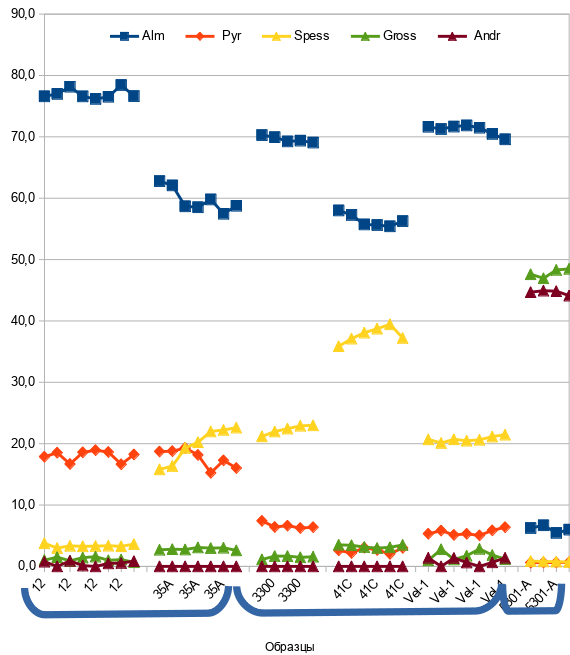
\includegraphics[width=1\textwidth]{authors/polzunenkov-fig2.png}
        \caption{Миналы изученных зёрен гранатов}
        \label{fig:polzunenkov-fig2}
    \end{minipage}
\hfill
    \begin{minipage}[h]{0.5\linewidth}
      \begin{center}
              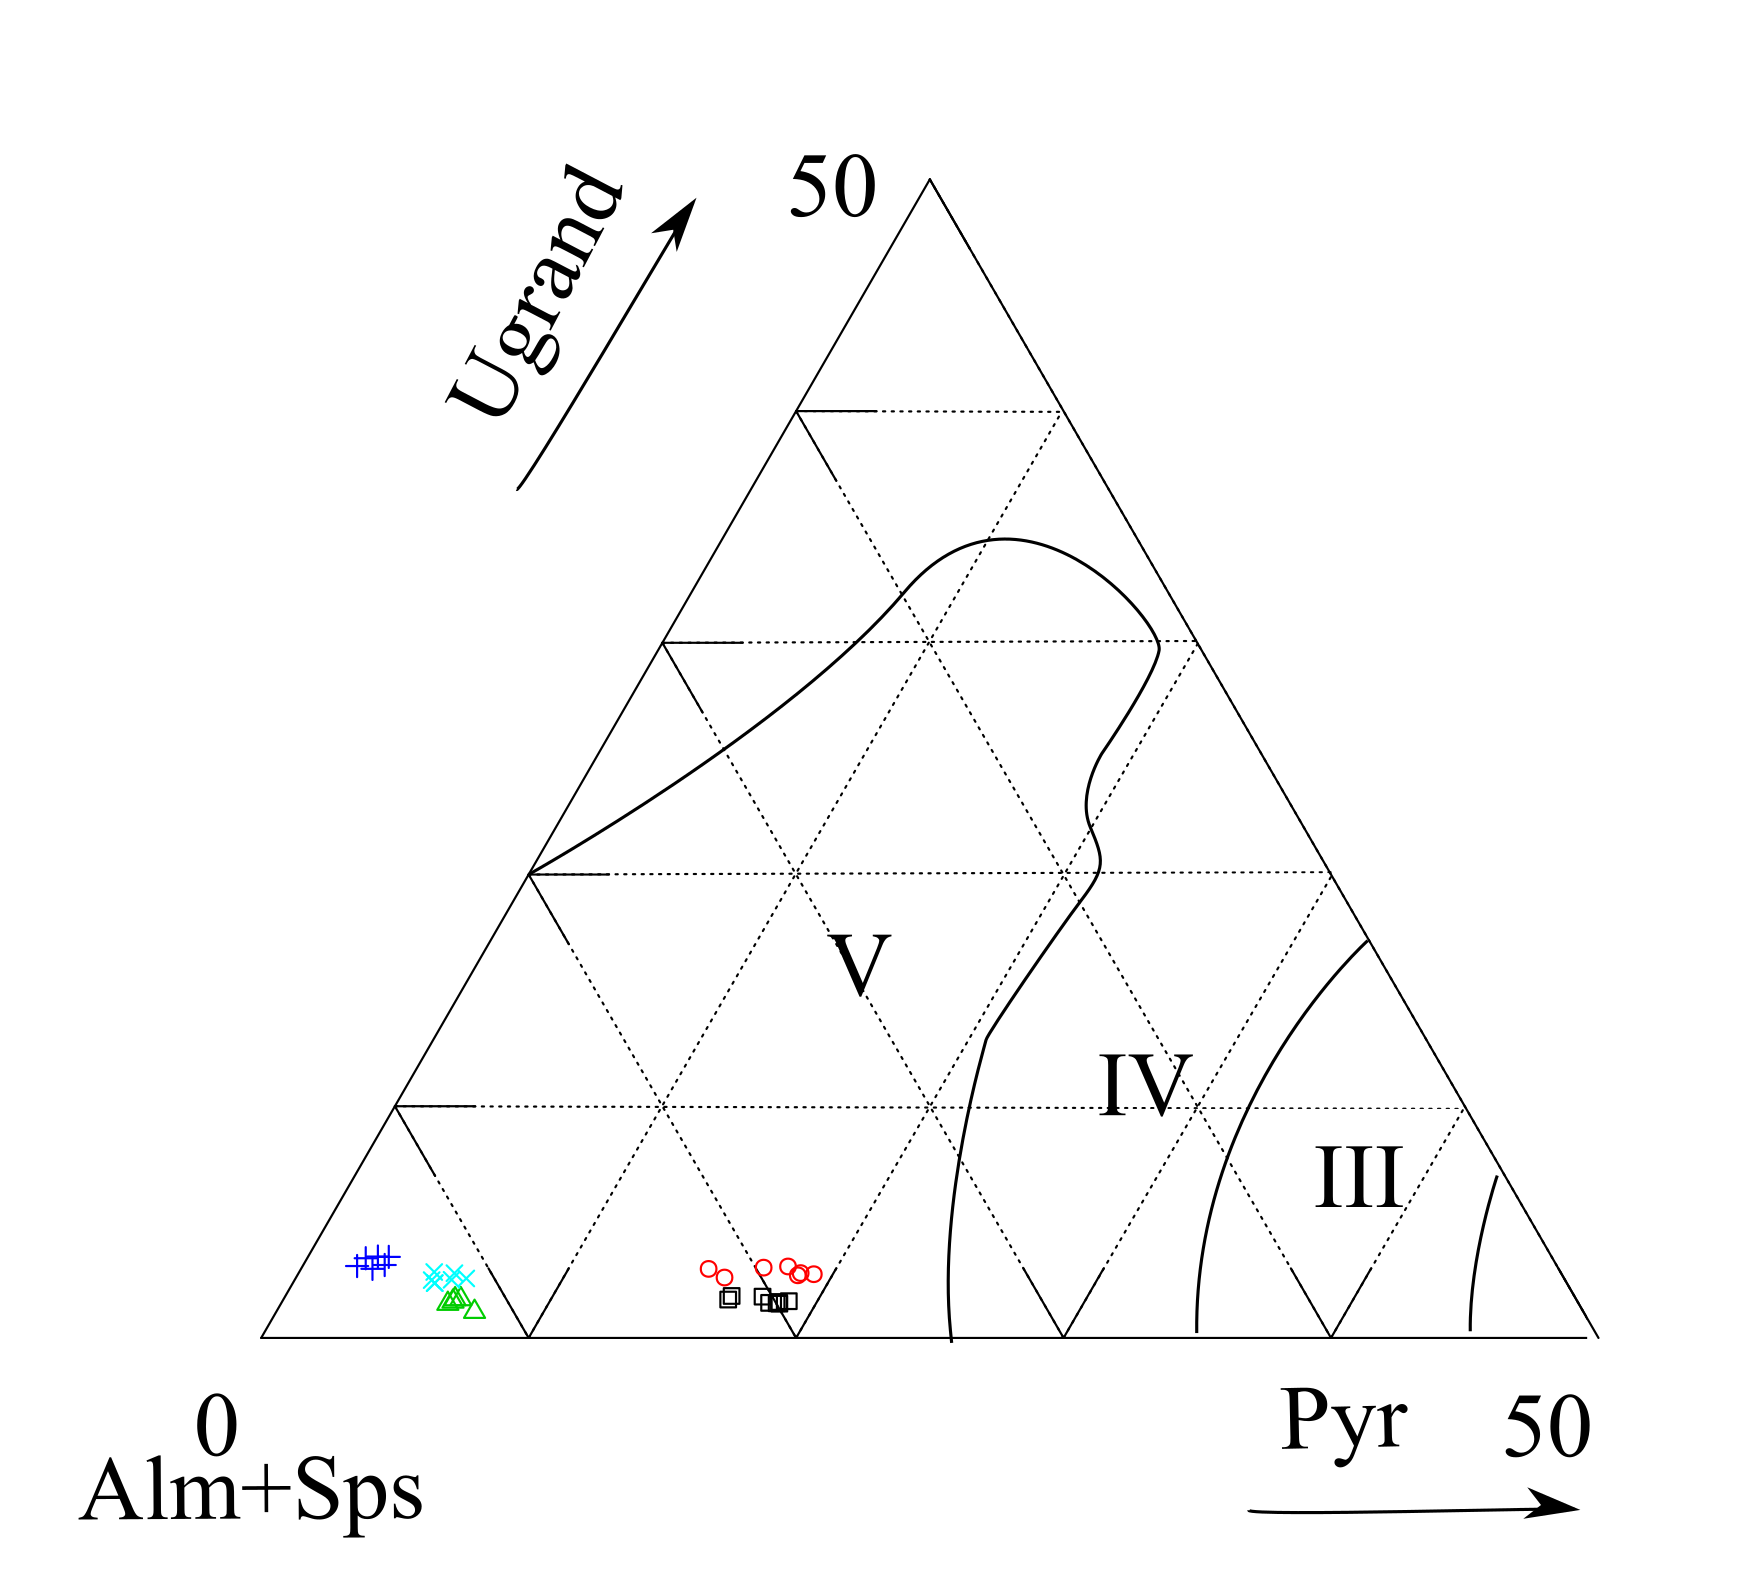
\includegraphics[width=1\textwidth]{authors/polzunenkov-fig3.png}
      \end{center}

        \caption{Состав гранатов на диаграмме А.\,И.~Сизых [3]. Поля составов граната: III~--- силлиманит-альмандин-ортоклазовой субфации,  IV~--- дистен-альмандин-мусковитовой  и  ставролит-дистен-альмандиновой субфации амфиболитовой фации, V~--- эпидот-амфиболитовой фации}
        \label{fig:polzunenkov-fig3}
    \end{minipage}


  \end{center}
\end{changemargin}

\end{figure}


Наличие в гранатовом габбро (обр. 5301A) гранатов с содержанием гроссулярового компонента $\sim$\,46\,\%  может указывать как на метасоматические изменения  вмещающих пород [1], так и на повышение давления при метаморфизме.  Согласно В.\,В.~Хлестову, за счёт  непрерывной  дегидратации во время длительного прогрессивного метаморфизма осадочных толщ, давление флюида  может превышать литостатическое давление [2].

Согласно минеральным термобарометрическим расчётам,  вмещающие неопротерозойские породы претерпели метаморфизм эпидот-амфиболитовой стадии при температуре 530--740\,\dgc (гранат-биотитовый термометр [3]), и давлениях $\sim$\,3,7~кбар  (барометр GASP [4], обр.\,12, метапелит). Антекристовая кристаллизация граната в гранитоидах Велиткенайского массива происходила при температуре не ниже 700\,\dgc. Оценки метаморфизма гранатового габбро требуют дополнительныйх исследований в части уточнения состава равновесных минеральных парагенезисов.
\clearpage
\begin{thebibliography}{99}
%1

\bibitem{}\BibAuthor{Добрецов Н. Л. и др.} Фации метаморфизма.~--- М.~: Недра, 1972.~--- 432~с.

\bibitem{}\BibAuthor{Перчук~Л.~Л., Лаврентьева~И.~В., Аранович~Л.~Я. и др.} Биотит-гранат-кордиеритовые равновесия и эволюция метаморфизма.~--- М.~: Наука, 1983.~--- 197~с.

\bibitem{}\BibAuthor{Сизых~А.\,И.} Докембрий Бирюсинского метаморфического пояса.~--- Иркутск~: Изд-во Иркут. ун-та, 1987.~--- 240~с.


\bibitem{}\BibAuthor{Holdaway, M. J.} Recalibration of the GASP geobarometer in light of recent garnet and plagioclase activity models and versions of the garnet-biotite geothermometer // American Mineralogist.~--- 2001.~--- Vol.~86.~--- P.~1117--1129.
\end{thebibliography}
\thispagestyle{empty}
